\subsection{Datasets} \label{sec:datasets}

\subsubsection{GulfStream OSSE}

\begin{figure}[t!]
\small
\begin{center}
\setlength{\tabcolsep}{2pt}
\begin{tabular}{ccc}
% $\mathcal X$ & $\hat \z = \bG_\theta(\x)$ & $\x = \bG_\theta^{-1} (\hat \z)$\\[0mm]
% NATL60&
% \multicolumn{2}{c}{\includegraphics[width=6.25cm,height=4.5cm]{content/figures/exp_natl60/psd_st/osse_2020a_psd_natl60}} 
% \\
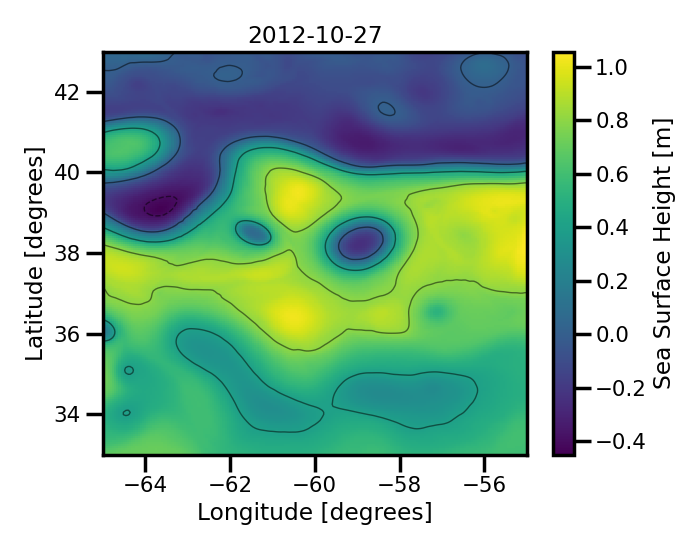
\includegraphics[width=4.25cm,height=3cm]{content/figures/maps/ssh/dc20a_nemo_ssh.png} &
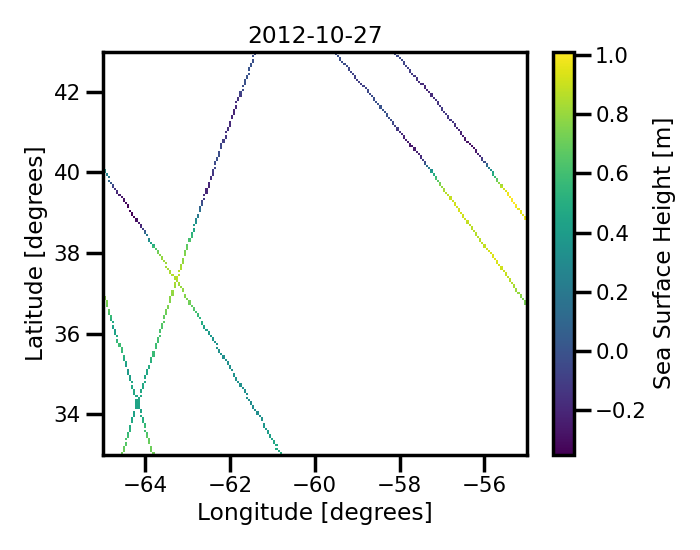
\includegraphics[width=4.25cm,height=3cm]{content/figures/maps/ssh/dc20a_nadir4_ssh.png} 
&
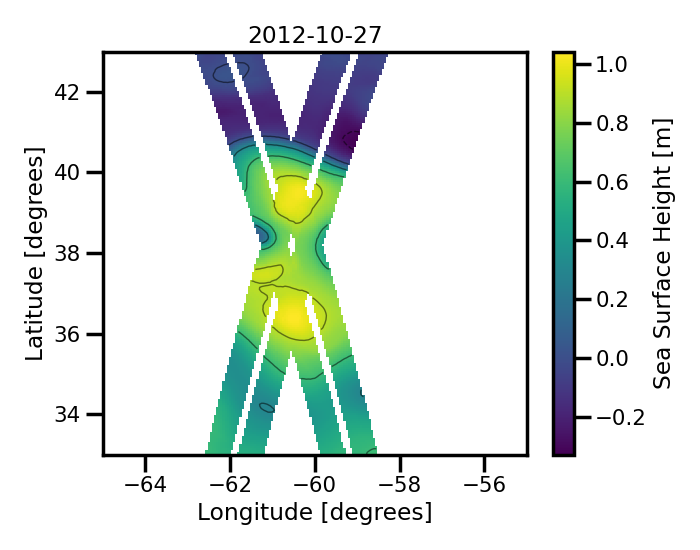
\includegraphics[width=4.25cm,height=3cm]{content/figures/maps/ssh/dc20a_swot1_ssh.png} 
% &
% 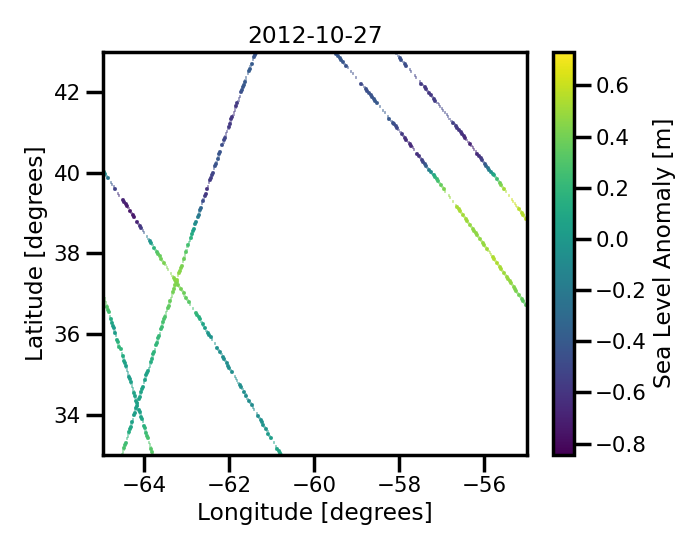
\includegraphics[width=6.25cm,height=4.5cm]{content/figures/maps/sla/dc20a_ssh_anomaly_nadir4_2012-10-27.png} 
\\
(a) NEMO Simulation & (b) NADIR Tracks &
(c) SWOT Tracks
\end{tabular}
% % \vspace{-4mm}
% \caption{Row I - Isotrophic PSD. Row 2 - Isotrophic PSD Score}
\caption{A snapshot at $27^{th}$ October, 2012 of the sea surface height (SSH) from the NEMO simulation for the OSSE experiment outlined in section~\ref{sec:data_challenges}. (a) showcases the full surface field and (b) showcases the aggregated alongtrack observations from the altimeters (12 hours before and 12 hours after).}
\vspace{-5mm}
\label{fig:maps}
\end{center}
\end{figure}

\subsubsection{GulfStream OSE}

\subsubsection{Mediterrenean OSE}

\subsubsection{GulfStream OSE}